\section{Consonância e dissonância}
\index{Música!Consonância}
\label{sec:consonancia}

\begin{tcbinformation}{Consonância (Música)}
\index{Música!Consonância}
\label{ref:consonancia}
Relação de tons soando agradáveis e estáveis ao ouvido \cite[pp. 26]{wright2012essential}.
Algumas combinações de teclas no piano produzem um som agradável e harmonioso.
\end{tcbinformation} 


\begin{tcbinformation}{Dissonância (Música)}
\index{Música!Dissonância}
\label{ref:dissonancia}
Relação de tons soando desagradáveis e instáveis ao ouvido \cite[pp. 26]{wright2012essential}.
Algumas combinações de teclas no piano produzem um som áspero e estridente.
\end{tcbinformation} 



A escola Pitagórica, que existiu no seculo VI (A.C.),
tentava compreender o universo;
com esse fim desenharam modelos matemáticos para explicar 
os fenômenos observados.
Entre os temas que foram tratados estava incluída a música,
e porquê alguns conjuntos de sons eram mais 
agradáveis de ouvir que outros \cite[pp. 11]{arbones2012armonia}.

Nos trabalhos feitos pela escola pitagórica
está incluído a criação de um instrumento chamado monocórdio;
este consta de uma única corda,
que tem um delimitador para modificar a longitude sem alterar a tensão nela \cite[pp. 12]{arbones2012armonia},
de modo que quando a corda do monocórdio é exitada o instrumento produz um som;
na Figura \ref{fig:consonancia}a podemos ver um modelo do monocórdio com a corda completa, 
que gera um som com frequência ``f''.
\begin{figure}[!h]
  \centering
    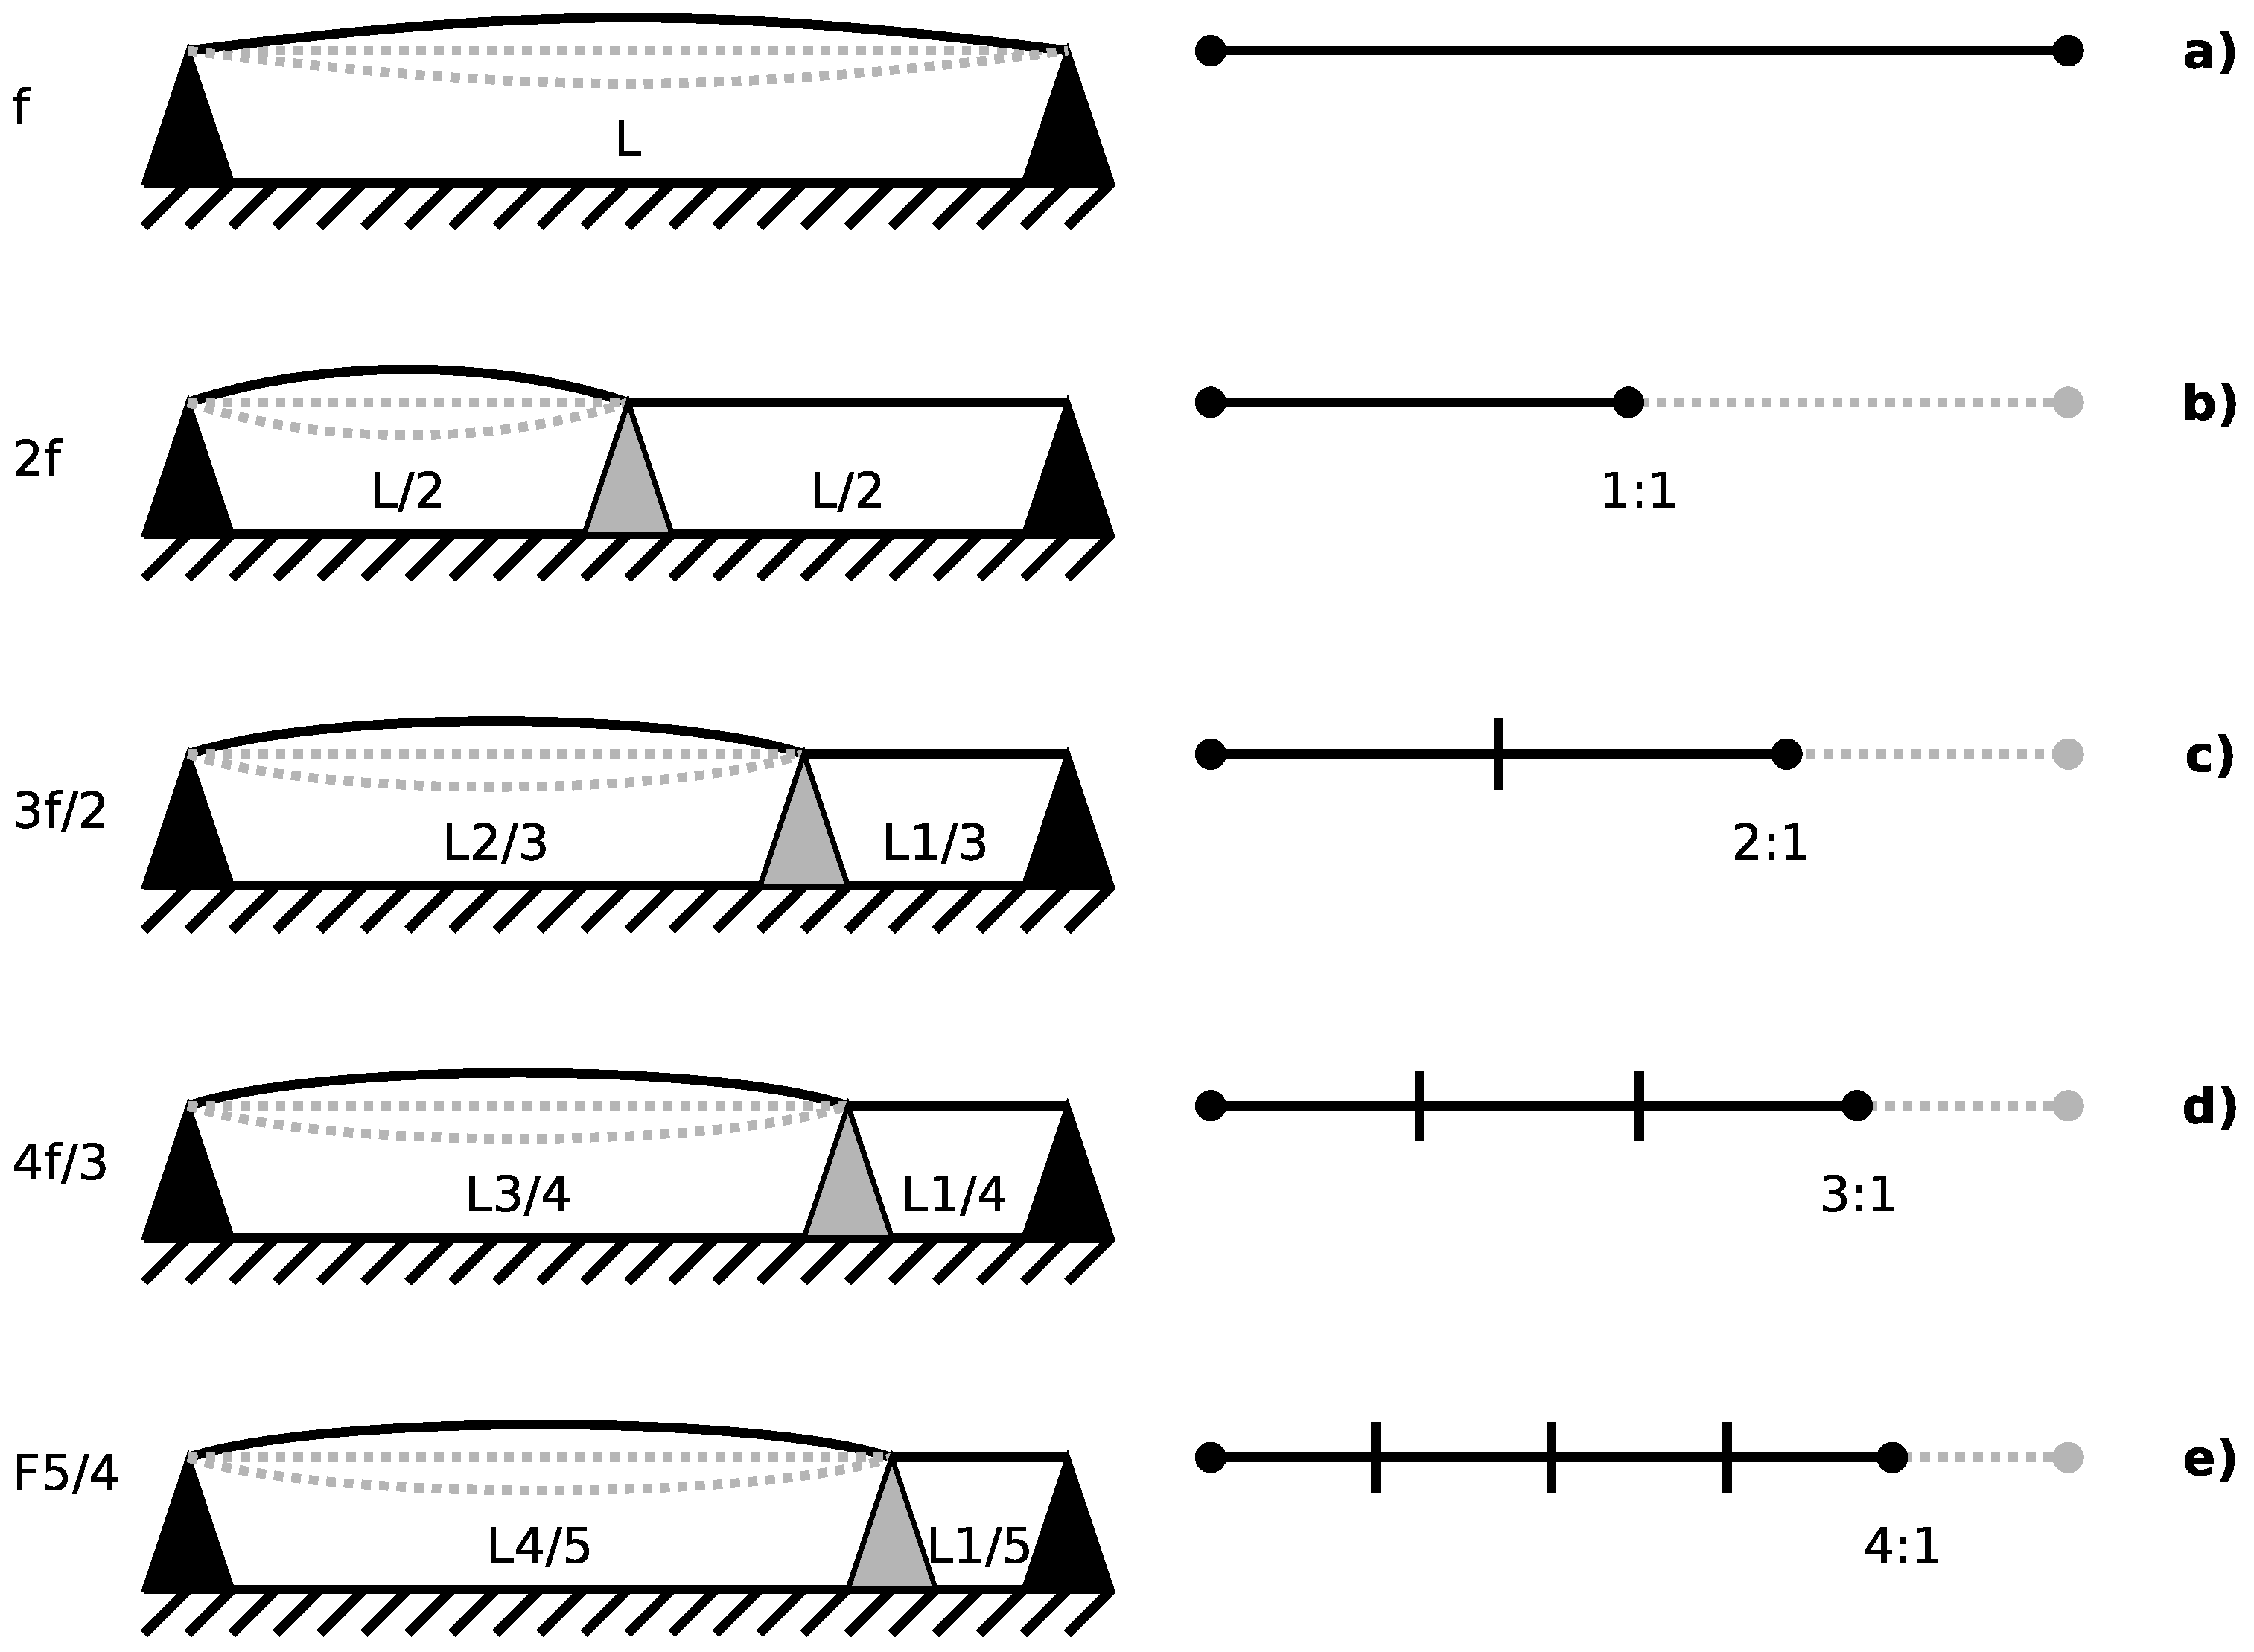
\includegraphics[width=0.85\textwidth]{chapters/cap-musica-composer/consonancia0.eps}
\caption{Consonância entre frequências.}
\label{fig:consonancia}
\end{figure}

Quando a longitude da corda no monocórdio diminui, 
a frequência do som gerado aumenta, é dizer se obtêm tons mais agudos.
Por conseguinte, na corda, longitude e frequência tem uma relação inversa \cite[pp. 12]{arbones2012armonia}. 
Entre os resultados obtidos com este instrumento, 
esteve a constatação de que alguns pares de longitudes na corda, em proporções especificas, 
geravam sons mais agradáveis de ouvir que outros 
ao ser executados ao mesmo tempo \cite[pp. 12]{arbones2012armonia}.
Assim, os pitagóricos descobriram que as proporções mais ``simples'' na corda executadas ao uníssono,
eram as que geravam os sons mais consonantes \cite[pp. 12]{arbones2012armonia}.

Nas Figuras \ref{fig:consonancia}[b - e], podemos ver algumas proporções de segmentos de corda,
como: 1:1, 2:1, 3:1 e 4:1; se exitamos os segmentos de longitudes maiores estas geram tons com frequências: 
$2$f, $\frac{3}{2}$f, $\frac{4}{3}$f e , $\frac{5}{4}$f.
A relação mais simples (1:1) provoca a duplicação da frequência (2f na Figura \ref{fig:consonancia}b)
quando comparado à frequência produzida pela corda completa (f). 
Na atualidade 
chamamos \hyperref[sec:pos:Oitava]{\textbf{oitava}} superior a uma nota com o dobro de frequência que a original. 
A seguinte em simplicidade é a proporção 2:1 que no segmento mais longo gera um som com uma frequência $\frac{3}{2}$f (Figura \ref{fig:consonancia}c);
na atualidade chamamos \textbf{intervalo de quinta} a esta proporção de frequências.
Nas Figuras \ref{fig:consonancia}[d-e] com frequências $\frac{4}{3}$f e , $\frac{5}{4}$f respetivamente,
a sensação de consonância com f diminui proporcionalmente à ``complexidade'' das frações destas frequências \cite[pp. 12]{arbones2012armonia}.

Por estas observações os pitagóricos concluíram que seriam consonantes com a frequência $f$, sons com uma frequência igual a 
\begin{equation}
\label{eq:simplespita}
\frac{n+1}{n}f,
\end{equation}
sendo que o nível de consonância diminui com o aumento de ``n'' \cite[pp. 14]{arbones2012armonia}.

\PRLsep{Escala diatônica}
\label{ref:paginadiatonicanumerica}

Se usamos as frequências da Equação \ref{eq:simplespita}, para $n=\{1,2,3,4\}$,
e multiplicamos estas frequências por $\frac{3}{2}$ ou $\frac{1}{2}$, que
são as proporções de frequência que geram maior consonância,
obteremos a \hyperref[sec:pos:Diatonica]{\textbf{escala diatônica}} (E.D.).
Esta escala pode ser comparada com a \hyperref[sec:pos:Cromatica]{\textbf{escala cromática}} (E.C.)
que está \hyperref[subsec:tempigual]{\textbf{igualmente temperada}}, 
como mostra a Tabela \ref{tab:pitagorascromatica}, onde é usada a nota musical ``dó'' 
como referencia na comparação (é dizer a \hyperref[sec:Tonica]{\textbf{tônica}}).
\begin{table}[h]
  \centering
  \begin{tabular}{|l|l|l|l|l|l|l|l|l|}
  \hline
  E. Diatônica  & dó & ré & mi & fá & sol & lá & si & dó \\ \hline
  \hline
  Freq. E.D.  & f  & $\frac{9}{8}$f & $\frac{5}{4}$f & $\frac{4}{3}$f & $\mathbf{\frac{3}{2}}$\textbf{f} & $\frac{5}{3}$f & $\frac{15}{8}$f & $\mathbf{2}$\textbf{f}\\ \hline
  E. Cromática & f  & $\alpha^{2}$f  & $\alpha^{4}$f  & $\alpha^{5}$f  & $\alpha^{7}$f  & $\alpha^{9}$f  & $\alpha^{11}$f  & $2$f\\ \hline \hline
  %%Error$\%$ &  0.0  & 0.23 & 0.79  & 0.11 & 0.11 & 0.91 & 0.68 & 0.0 \\ \hline
  Error$\%$ &  0.00 & 3.91 &-13.69 &-1.96 & 1.96 &-15.64&-11.73& 0.00 \\ \hline
  \end{tabular}
  \caption{Relação de frequências, usando $\alpha=2^\frac{1}{12}$.}
  \label{tab:pitagorascromatica}
\end{table}

É possível ver que existe uma ligeira diferença numérica, 
entre as proporções de frequências na escala diatônica baseada nas consonâncias descobertas pela escola pitagórica,
e as proporções de frequência de nossa atual escala cromática igualmente temperada,
no menor dos casos temos um  erro na frequência de $1.96\%$ de um \hyperref[sec:pos:Semitom]{\textbf{semitom}}, 
e no pior dos casos um erro de $15.64\%$.

\PRLsep{Análises objetivo}
Fora da subjetiva perspetiva da escola pitagórica, 
em indicar que frações mais simples na frequência geram sons consonantes; 
existem motivos objetivos para fundamentar esta afirmação.

Na Figura \ref{fig:corda32} vemos as sinais $y_{f}$ e $y_{\frac{3}{2}f}$, 
produzidas pelos sons com frequências $f=1000$hz e $\frac{3}{2}f$,
correspondentes as cordas de longitude $L$ e $\frac{2}{3}L$ respetivamente;
é interessante observar que se precisam dois ciclos completos da sinal $y_{f}$,
para que ambas sinais voltem a estar em sincronia e que a sinal soma, $y_{f}+y_{\frac{3}{2}f}$, forme um ciclo completo.


Na mesma linha de análises, na Figura \ref{fig:corda53} observamos as sinais $y_{f}$ e $y_{\frac{5}{3}f}$, 
produzidas pelos sons com frequências $f=1000$hz e $\frac{5}{3}f$,
correspondentes as cordas de longitude $L$ e $\frac{3}{5}L$ respetivamente;
similarmente ao caso anterior, observamos que se precisam três ciclos completos da sinal $y_{f}$,
para que ambas sinais voltem a estar em sincronia e que a sinal soma, $y_{f}+y_{\frac{5}{3}f}$, forme um ciclo completo.

\begin{figure}
    \centering
    \begin{subfigure}[b]{0.8\textwidth}
        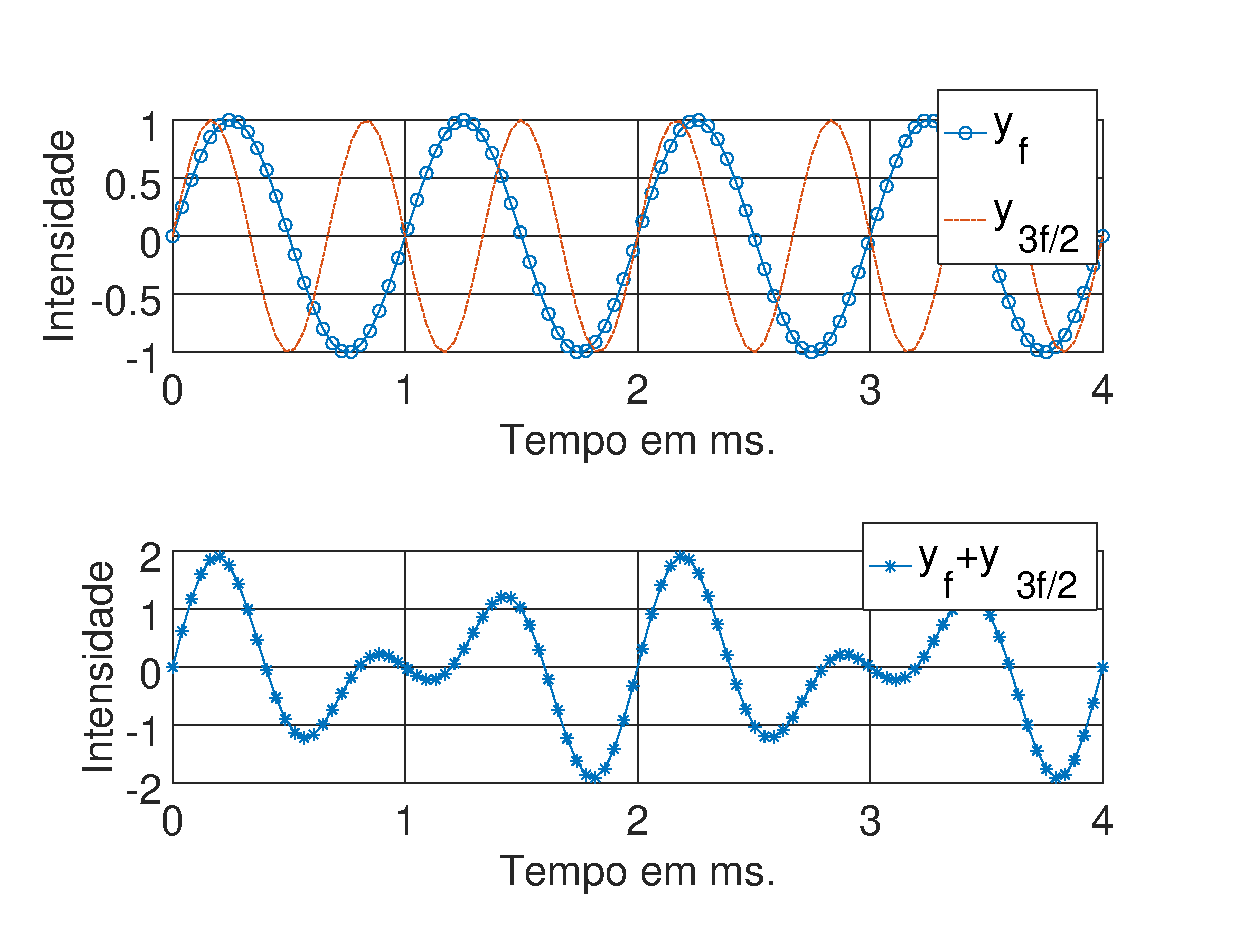
\includegraphics[width=\textwidth]{chapters/cap-musica-composer/consonancia32.eps}
        \caption{Consonância entre sinais com frequências $f$ e $\frac{3}{2}f$}
        \label{fig:corda32}
    \end{subfigure}
    ~ %add desired spacing between images, e. g. ~, \quad, \qquad, \hfill etc. 
      %(or a blank line to force the subfigure onto a new line)
    \begin{subfigure}[b]{0.8\textwidth}
        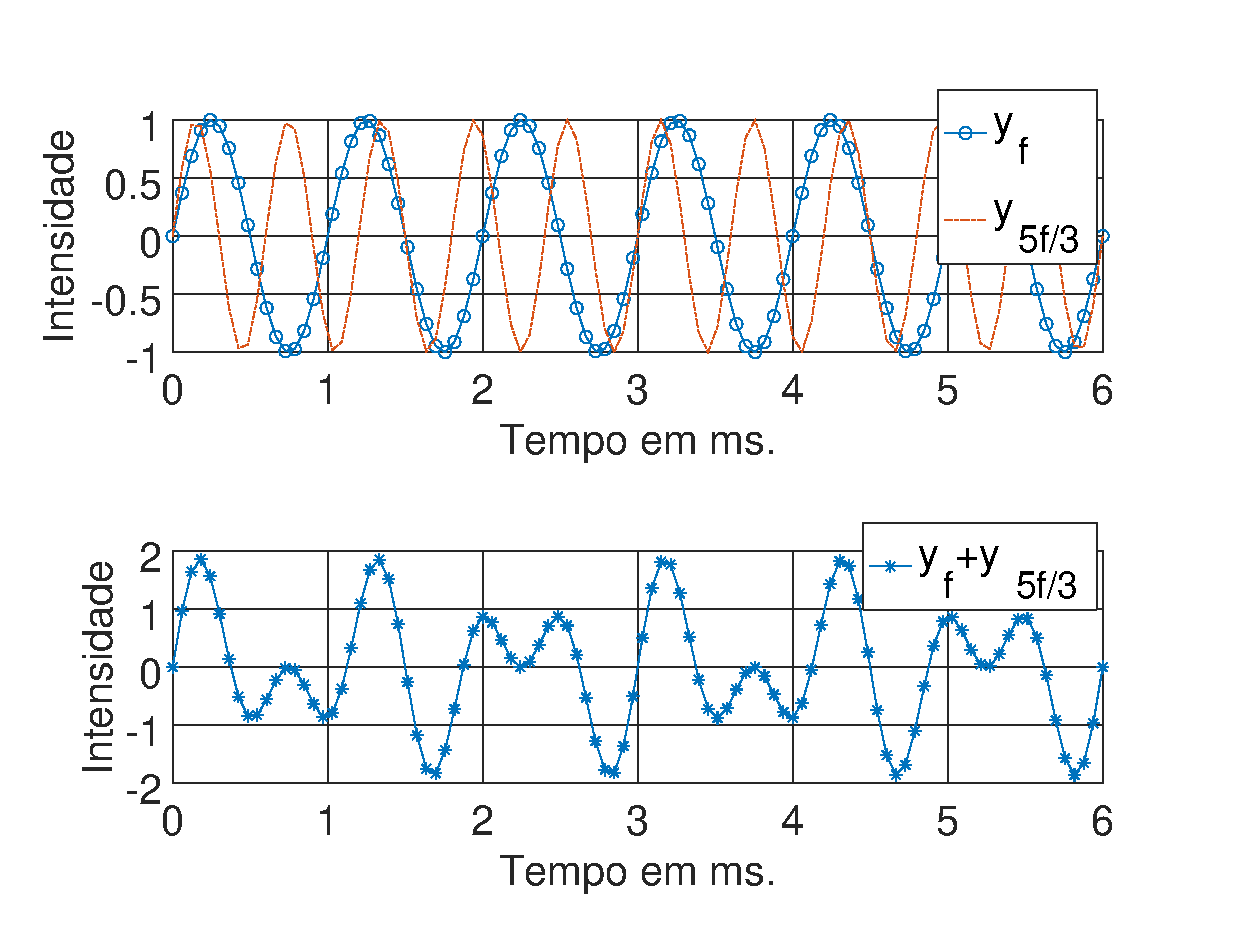
\includegraphics[width=\textwidth]{chapters/cap-musica-composer/consonancia53.eps}
        \caption{Consonância entre sinais com frequências $f$ e $\frac{5}{3}f$}
        \label{fig:corda53}
    \end{subfigure}
\caption{Analises de consonância.}
\label{fig:consonanciaper}
\end{figure}

Assim, deduzimos que pela forma fraccionaria e relativa das frequência nas sinais, 
podemos usar o denominador da fração na frequência,
para conhecer quantos ciclos debem passar para que a ambas sinais em estudo voltem a estar em sincronia;
de modo que seremos capazes de relacionar um estado de maior nível de dissonância (N.D.) com um maior número de ciclos.
A Tabela \ref{tab:pitagorascromatica2} mostra estas relações, 
porém foram agregadas as letras ``a'' e ``b'' para indicar menor e maior dissonância respetivamente,
nos casos com igual N.D., este critério foi aplicado tomando em conta que a escala
que comumente temos num piano está igualmente temperada,
é como vimos na Tabela  \ref{tab:pitagorascromatica},
existe um erro de aproximação a estas frações;
de modo que foi colocada a etiqueta de ``b'' ao caso de maior erro e a etiqueta de ``a'' ao de menor.
\begin{table}[h]
  \centering
  \begin{tabular}{|l|l|l|l|l|l|l|l|l|}
  \hline
  E. Diatônica    & dó & ré & mi & fá & sol & lá & si & dó \\ \hline
  \hline
  Semitons E.C.   & 0  & 2  & 4  & 5  & 7  & 9  & 11 & 12 \\ \hline
  Freq. E.D.  & f  & $\frac{9}{8}$f & $\frac{5}{4}$f & $\frac{4}{3}$f & $\mathbf{\frac{3}{2}}$\textbf{f} & $\frac{5}{3}$f & $\frac{15}{8}$f & $\mathbf{2}$\textbf{f}\\ \hline \hline
  N.D. &  0 & 8a & 4 & 3a & 2 & 3b & 8b & 1 \\ \hline
  \end{tabular}
  \caption{Nível de dissonância com a nota musical dó.}
  \label{tab:pitagorascromatica2}
\end{table}

\begin{example}
Com a ajuda de um piano, que esteja igualmente temperado,
use a nota dó como referencia e comprove o nível de consonância com todas as demais notas musicais;
verifique se concorda com o mostrado na Tabela \ref{tab:pitagorascromatica2}.
\end{example}~

\PRLsep{Conclusões}

Finalmente, podemos concluir que existe uma maior consonância entre
\begin{itemize} 
\item os tons com frequências $f$ e $2f$, e 
\item os tons com frequências $f$ e $\frac{3}{2}f$;
\end{itemize}
para outros valores de frequência, 
como entre $f$ e $\frac{4}{3}f$, o nível de consonância diminui  
 gradualmente com o aumento da complexidade das frações nas frequências.

Na música atual, as relações de consonância são usadas na escala cromática, 
em notas musicais com:
\begin{itemize} 
\item Uma oitava de diferença, para as frequências relacionadas como $f$ e $2f$, 
por exemplo: dó e dó'.
\item Um intervalo de quinta, sete semitons, para frequências relacionadas como  $f$ e $\frac{3}{2}f$, 
por exemplo: dó e sol. Porém, numa escala igualmente temperada, 
os 7 semitons (1.4983) são uma aproximação\footnote{Sim, você está supondo certo,
toda a música atual está ligeiramente ``desafina'', pois usa uma aproximação para a consonância.}
 da fração $\frac{3}{2}$.
\end{itemize}~


Os seres humanos não nos sentimos confortáveis ao terminar o dia com um argumento não resolvido; 
da mesma forma, não apreciamos terminar nossa música com uma dissonância não resolvida \cite[pp. 26]{wright2012essential}.

\begin{comment}
https://www.youtube.com/watch?v=54KuXjjzqVA

Jaime Altozano:

A tensão e o desconforto pode ser gerado por dissonancia, porém não é o unico fator,
por exemplo influencia tambem o ataque (ou seja que tanto demora a nota em chegar a seu apice violin lento vs. piano)
e tambem o timbre (timbre de flauta vs. timbre de piano)
\end{comment}

